\documentclass[hyperref={pdfpagelabels=false}]{beamer}
\usepackage{listings}
\usepackage{color}
\usepackage[utf8x]{inputenc}
\usepackage[ngerman]{babel}
\usepackage{hyperref}
\usepackage{tikz}
\usepackage{svg}
\usepackage{setspace}
\usepackage{lmodern}
\usepackage{subcaption}

\usepackage{caption}
% redefines the caption setup of the figures environment in the beamer class.
\captionsetup[figure]{labelformat=empty}

%%
% Quellen
%%

% https://bitcoin.org/en/developer-reference
% Blockchain Basics

%\usepackage{csquotes}
%\MakeOuterQuote{"}

\usepackage{amsmath}

%% Fonts
\usepackage[default]{sourcesanspro} %% HTWK Font
%\usepackage[familydefault,regular]{Chivo}
%\usepackage[sfdefault,lf]{carlito}
%\usepackage[sfdefault]{cabin}
%\usepackage[sfdefault]{GoSans}

%\usepackage[T1]{fontenc}

\usetheme{Dresden}


\definecolor{primary}{HTML}{37354b}
%\definecolor{primary}{HTML}{3a393f}

%\definecolor{accent}{HTML}{990097}
%\definecolor{accent}{HTML}{0066ce}
\definecolor{accent}{HTML}{0ec6b2}

\setbeamercolor*{structure}{bg=accent,fg=primary}

\setbeamercolor*{palette primary}{use=structure,fg=white,bg=structure.fg}
\setbeamercolor*{palette secondary}{use=structure,fg=white,bg=structure.fg}
\setbeamercolor*{palette tertiary}{use=structure,fg=white,bg=structure.fg!115}
\setbeamercolor*{palette quaternary}{fg=white,bg=black}

\setbeamercolor{section in toc}{fg=black,bg=white}
\setbeamercolor{alerted text}{use=structure,fg=structure.fg!50!black!80!black}

\setbeamercolor{titlelike}{parent=palette primary,fg=structure.fg!50!black}
\setbeamercolor{frametitle}{use=structure,bg=white,fg=structure.fg!90}

\setbeamercolor{block title}{bg=structure.bg!0,fg=structure.bg!80!black}

%\addtobeamertemplate{block begin}{\vspace{-0.5cm}}{}
%\addtobeamertemplate{block end}{}{\vspace{-0.5cm}}


\setbeamertemplate{itemize item}{\color{accent}$\blacksquare$}
\setbeamertemplate{itemize subitem}{\color{accent}$\blacktriangleright$}

\setbeamertemplate{footline}
  {%
  \begin{beamercolorbox}[colsep=1.5pt]{upper separation line foot}
  \end{beamercolorbox}
  \begin{beamercolorbox}[ht=2.5ex,dp=1.125ex,%
    leftskip=.3cm,rightskip=.3cm plus1fil]{author in foot}%
    \leavevmode{\usebeamerfont{author in head/foot}\insertshortauthor}%
    \hfill%
    {\usebeamerfont{institute in foot}\usebeamercolor[fg]{institute in foot}\insertshortinstitute}%
  \end{beamercolorbox}%
  \begin{beamercolorbox}[ht=2.5ex,dp=1.125ex,%
    leftskip=.3cm,rightskip=.3cm plus1fil]{title in foot}%
    {\usebeamerfont{title in head/foot}\insertshorttitle}\hfill{\usebeamercolor[fg]{page number in head/foot}\usebeamerfont{page number in head/foot}\usebeamertemplate{page number in head/foot}}%
  \end{beamercolorbox}%
  \begin{beamercolorbox}[colsep=1.5pt]{lower separation line foot}
  \end{beamercolorbox}
}

\setbeamercolor{title in foot}{use=structure,bg=structure.fg!110,fg=white}
\setbeamercolor{author in foot}{bg=accent,fg=black}
%\setbeamercolor{institute in foot}{bg=accent,fg=black}

\setbeamercolor*{titlelike}{parent=palette primary}

\newcommand{\putat}[3]{\begin{picture}(0,0)(0,0)\put(#1,#2){#3}\end{picture}}
\newcommand{\shortblock}{\vspace*{-0.9\baselineskip}}

\title {Hieroglyph Localization and Recognition}
\subtitle{Modul Objekt- und Gestenerkennung}
\author {Jan Oelschlegel, Michael Schmidt}
\institute{HTWK Leipzig, Fakultät IM}
\date{\today} 

\begin{document}

\maketitle


\section{Datenquellen}

\begin{frame}{Ziel}
	\begin{itemize}
		\item Lokalisierung und Erkennung von Hieroglyphen
		\item Sicherstellen der korrekten Reihenfolge
	\end{itemize}

	%columns

	\begin{columns}
		\begin{column}{0.5\textwidth}
			\begin{figure}[h]
				\begin{subfigure}{0.3\textwidth}
					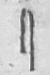
\includegraphics[width=0.9\linewidth, height=2cm]{img/200000_S29.png}
					\caption{S29}
					\label{fig:s29}
				\end{subfigure}
				\begin{subfigure}{0.3\textwidth}
					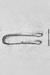
\includegraphics[width=0.9\linewidth, height=2cm]{img/200001_V13.png}
					\caption{V13}
					\label{fig:v13}
				\end{subfigure}
				\begin{subfigure}{0.3\textwidth}
					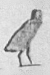
\includegraphics[width=0.9\linewidth, height=2cm]{img/200003_G43.png}
					\caption{G43}
					\label{fig:g43}
				\end{subfigure}
				\caption{}
				\label{fig:img}
			\end{figure}
		\end{column}
		\begin{column}{0.5\textwidth}
			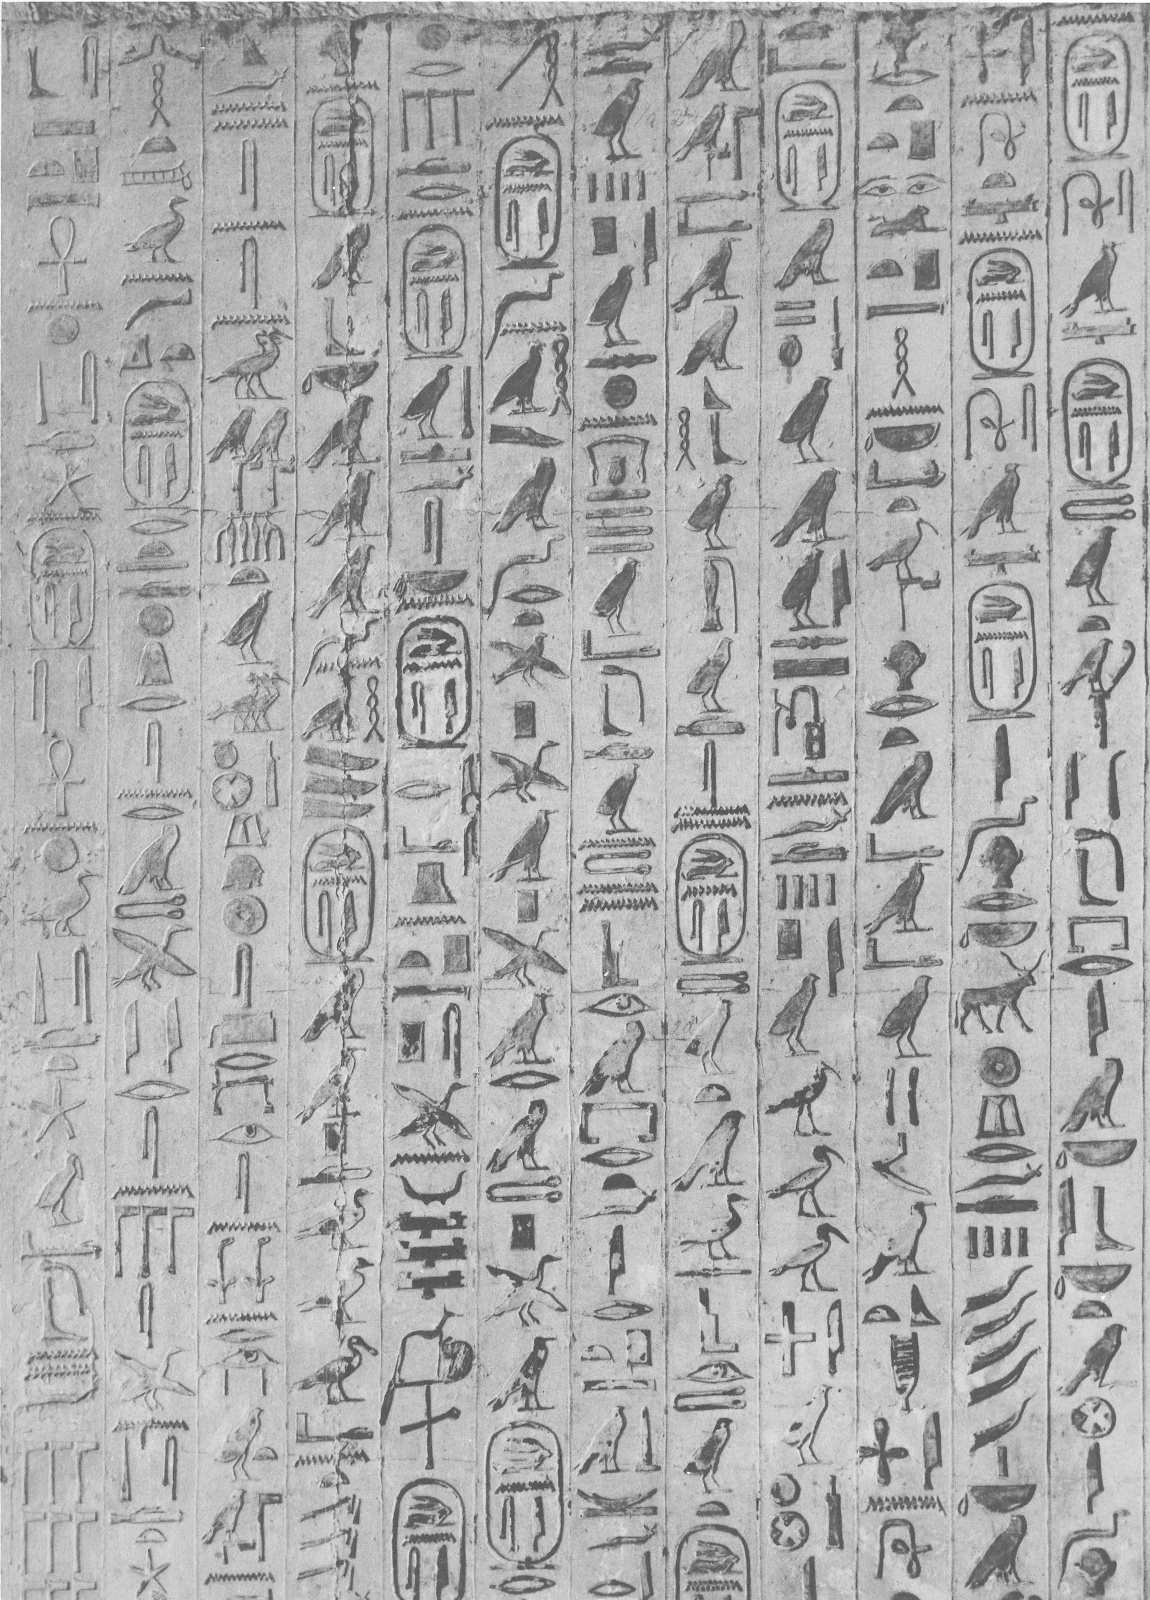
\includegraphics[width=0.7\linewidth]{img/egyptianTexts3.jpg}
		\end{column}
	\end{columns}
\end{frame}

\begin{frame}{Datenquellen}
	\begin{columns}
		\begin{column}{0.5\textwidth}
			\begin{itemize}
				\item Hieroglyphen der Unas-Pyramide
				      \begin{itemize}
					      \item 4210 Einzelbilder
					      \item 171 verschiedene Hieroglyphen
				      \end{itemize}
				\item Synthetisierte Hieroglyphen
			\end{itemize}
		\end{column}
		\begin{column}{0.5\textwidth}  %%<--- here
			\begin{center}
				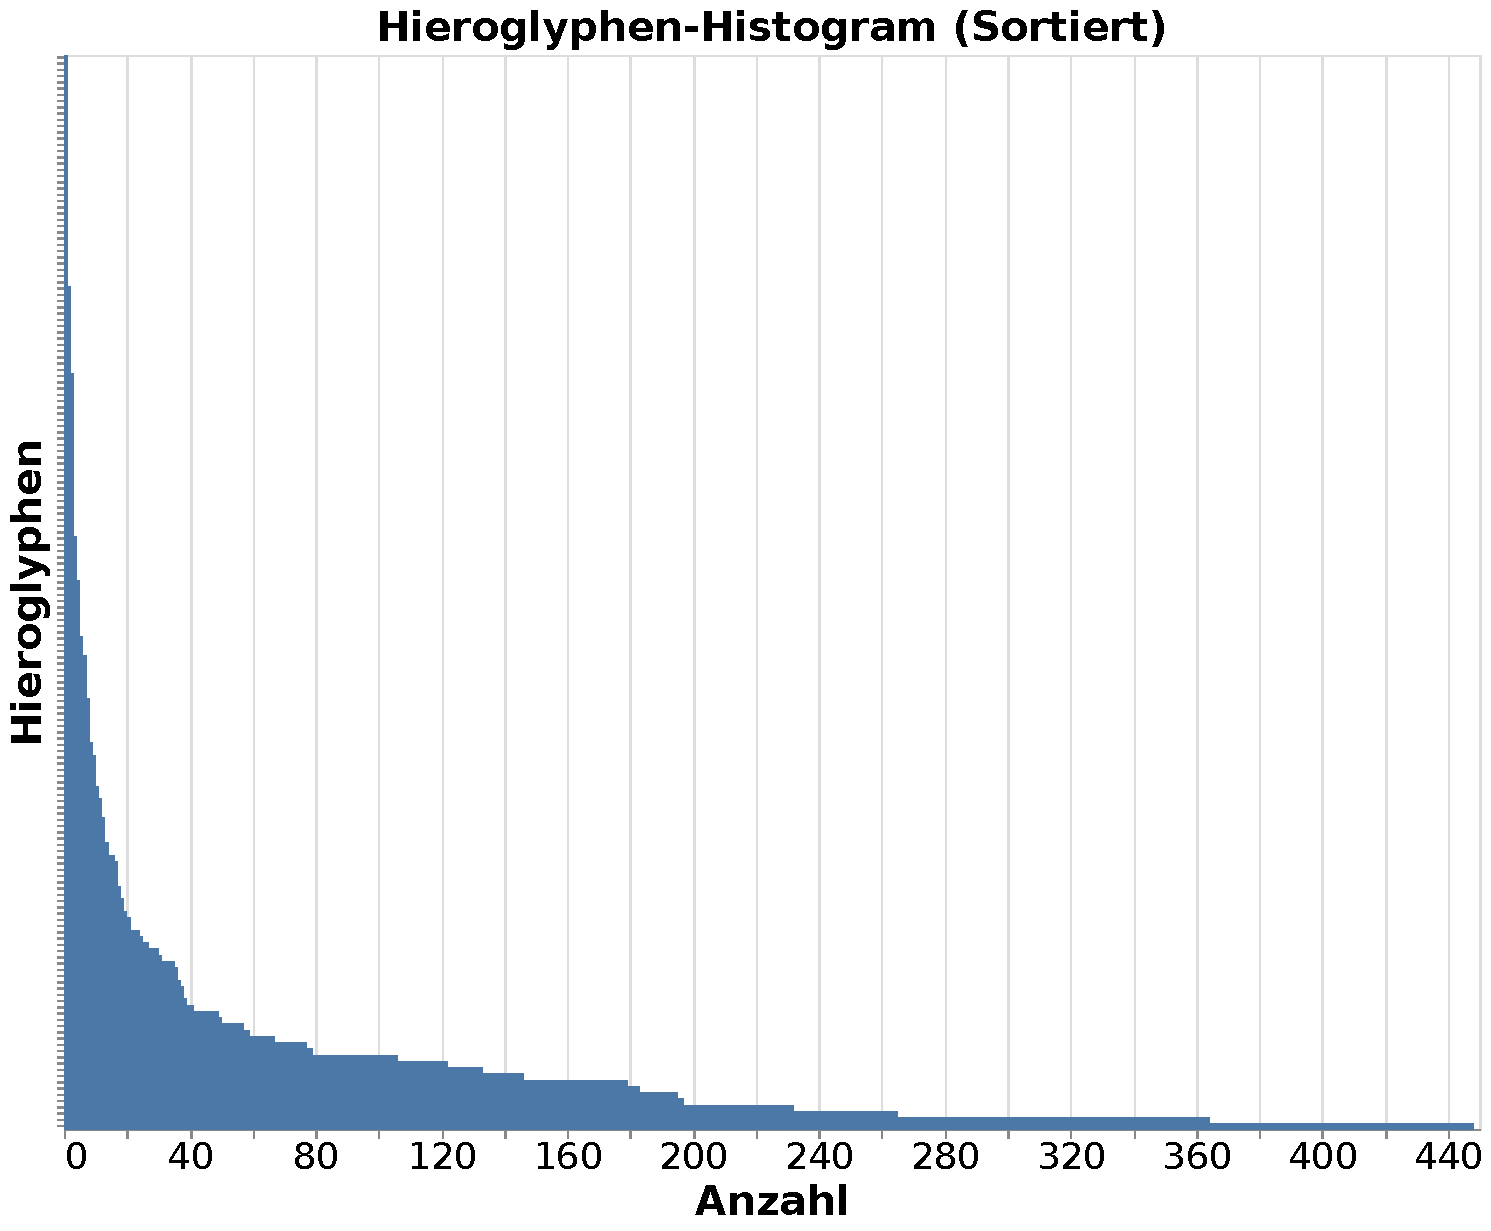
\includegraphics[width=1\textwidth]{img/dia.pdf}
			\end{center}
		\end{column}
	\end{columns}
\end{frame}

\end{document}
